\documentclass[10pt]{scrartcl}
\usepackage{amsmath,amsthm,amssymb,mathtools,xfrac}
\usepackage{enumerate}
\usepackage[utf8]{inputenc}
%\usepackage{german}
\usepackage{a4wide}
\usepackage{graphics}
\usepackage{graphicx}
\usepackage[T1]{fontenc}
\usepackage{epsfig}
\usepackage{libertine}
\usepackage[pdftex]{hyperref}
\usepackage{refcount}
\usepackage{framed}
\usepackage{xcolor}
\usepackage{multicol}
\usepackage{enumitem}
\usepackage{caption}
\usepackage{gensymb}
\usepackage[export]{adjustbox}
\usepackage{booktabs}

\topmargin-.5in \textheight9in \oddsidemargin0in \textwidth6.5in

% General definitions
\newcommand{\lat}{\theta}
\newcommand{\colat}{\tilde \theta}

\begin{document}


\begin{minipage}{.5\textwidth}
{\scshape Department of Mathematics and Informatics \\
University of Cologne\\}
\small Prof. Dr. Gregor Gassner \\
\small Dr. Andrés Rueda-Ramírez \\
\end{minipage}
\hfill
\begin{minipage}{.3\textwidth}
\begin{flushright}

\includegraphics[width=3cm]{figs/logo-uni-koeln.jpg}\\
\today
\end{flushright}
\end{minipage}

\begin{center}
{\Large\bfseries
An Introduction to Climate Modeling}\\
\vspace{0.2cm}
{\bfseries Milestone 2 - Albedo, Solar Forcing and Visualization in Time}
\end{center}


\section{Compute Albedo and Solar Forcing Terms and Visualize in Time}

In milestone 2 you will program the calculation of all necessary parameters for the calculation of the time and space dependent solar forcing and then visualize it as an animation over a period of one year in 48 time steps. For this you will need the functions \small\texttt{\detokenize{read_geography}} \normalsize and \small\texttt{\detokenize{robinson_projection}} \normalsize from milestone 1.

\begin{enumerate}
\item Write a function \small\texttt{\detokenize{calc_albedo}} \normalsize which outputs the albedo $\alpha_{ij}$ for the points $\left(\lat_i,\varphi_j\right)$ as a matrix $A \in \mathbb{R}^{65\times 128}$ depending on the earth surface type $T\in \mathbb{N}^{65\times 128}$ (see milestone 1). For the calculation use the albedo scheme below as proposed by Zhuang et al. \footnote{K. Zhuang, G.R. North, M.J. Stevens, {\em A NetCDF version of the two-dimensional energy balance model based on the full multigrid algorithm}, SoftwareX, Vol. 6, pp. 198-202, July 7, 2017.}.
\end{enumerate}

\begin{table}[!h]
\begin{center}
\begin{tabular}{lll}
\toprule
\textbf{Land mask} & \textbf{Albedo}   &                                                                                                 \\
\midrule
Land               & $0.30+0.12P_2(x)$ & $P_2(x)=\frac{(3x^2-1)}{2}$ for $x=\sin(\lat)$, where $\lat$ is the latitude in radians\\
Ocean              & $0.29+0.12P_2(x)$ &                                                                                                 \\
Sea ice            & $0.60$            &                                                                                                 \\
Snow               & $0.75$            &                                                                                                 \\
\bottomrule
\end{tabular}
\end{center}
\end{table}

\begin{enumerate}
\item[2.] In the table below, besides atmospheric parameters, constants are given for each type of the earth's surface, which are used for the calculation of the effective heat capacity. The effective heat capacity of a grid cell results from the sum of the heat capacity of the respective surface type and the heat capacity of the overlying atmospheric column. Since the climate model measures time in years, this heat capactiy has to be divided by the number of seconds in a year $3.15576\times10^7 s$. Implement a function \small\texttt{\detokenize{calc_heatcapacity}} \normalsize analogous to $\small\texttt{\detokenize{calc_albedo}}$ to calculate the geography-dependent heat capacity per surface area using the given constants from the table below.
\end{enumerate}

\begin{table}[!h]
\small
	\begin{center}
	\begin{tabular}{p{2.5cm}p{2cm}p{5cm}p{2cm}}
	\toprule
	\textbf{Types} & \textbf{Density $\rho$ in $\mathrm{kg\,m}^{-3}$} & \textbf{Specific heat capacity in $\mathrm{J\,kg^{-1}K^{-1}}$} &  \textbf{Depth in $\mathrm{m}$}\\
	\midrule
	\text{Atmosphere}&1.225 & 1000 & 3850 \\
	\text{Ocean mixed layer}& 1030 & 4000 & 70 \\
	\text{Sea ice}& 917 & 2000 & 1.5 \\
	\text{Land}& 1350 & 750 & 1.0 \\
	\text{Snow}& 400 & 880 & 0.5  \\
	\bottomrule
	\end{tabular}
%\caption{Surface-specific model parameters in the Klimakoffer.}
	\end{center}
\end{table}


\begin{enumerate}
\item[3.] Implement a function \small\texttt{\detokenize{read_true_longitude}} \normalsize to read in the true longitude $\lambda$ for each time step from the input file \small\texttt{\detokenize{True_Longitude.dat}} \normalsize and output it as a vector $\lambda \in \mathbb{R}^{48}$.

\item[4.] Write a function \small\texttt{\detokenize{insolation}}  \normalsize that calculates the insolation $S\left(\lat,t\right)$ as in Berger \footnote{A. L. Berger, {\em Long-Term Variations of Daily Insolation and Quaternary Climatic Changes}, Journal of the Atmospheric Sciences, Vol. 35, pp. 2362-2367, 1987.}. Input arguments of the function should be:
\begin{itemize}
\item $\theta$: latitude,
\item $S_0$: solar constant,
\item $e$: eccentricity,
\item $\epsilon$: obliquity,
\item $\tilde \omega$: precession distance,
\item $\lambda$: true longitude.
\end{itemize}

The insolation at latitude $\lat$ and time $t$ is given by:
\begin{align*}
S(\lat,t) =
\begin{cases}
0 & \text{for $(\lat,t)$ without sunrise}, \\
S_0\rho(t) \sin (\lat) \sin \big(\delta(t)\big) & \text{for $(\lat,t)$ without sunset}, \\
\frac{S_0 \rho(t)}{\pi}\Big(H_0(t) \sin (\lat) \sin \big(\delta(t)\big) + \cos (\lat) \cos \big(\delta(t)\big) \sin \big(H_0(t)\big)\Big) & \text{else}, \\
\end{cases}
\end{align*}
where $\delta(t)$ is the declination of the sun with
\begin{align*}
\sin(\delta(t)) = \sin(\epsilon)\sin (\lambda(t)).
\end{align*}
Here, $\rho$ is the normalized distance between earth and sun squared,
 \begin{align*}
 \rho(t) =  \left(\frac{1 - e \cos (\nu(t))}{1-e^2}\right)^2,
 \end{align*}
with eccentricity $e$ and the positional angle of the Earth on its orbit around the Sun $\nu(t)=\lambda(t)-\tilde \omega$ as given counterclockwise from aphelion.
\begin{align*}
H_0(t)= \arccos\big(-\tan(\lat) \tan(\delta(t))\big)
\end{align*}
describes the absolute angle of the sun at sunrise and sunset.
Make sure that your implementation handles values $\pm \infty$ of the tangent at the poles correctly.

\item[5.] Write a function \small\texttt{\detokenize{calc_solar_forcing}} \normalsize with input arguments
\begin{itemize}
	\item albedo values at the grid points,
	\item $S_0$: solar constant with default value $S_0 = 1371.685$,
	\item $e$: eccentricity with default value $e = 0.01674$,
	\item $\epsilon$: obliquity with default value $\epsilon  = 0.409253$,
	\item $\tilde \omega$: precession distance with default value $\tilde \omega = 1.783037$,
	\item $\left(\lambda_j\right)_{j = 1}^{n_t} \in \mathbb{R}^{n_t}$: true longitude for each time step.
\end{itemize}

Note that these default orbital parameters correspond to the year 1950.
This function should calculate and return the solar forcing $S_{sol}(\lat_i,\varphi_j,t_k)$ at each grid point $(\lat_i, \varphi_j)$ and for each time step $t_k$.
The return value should be a three-dimensional array, where the first dimension corresponds to the latitude, the second to the longitude, and the third to the time step.
The solar forcing is given by
\begin{equation*}
	S_\text{sol}\left(\lat,\varphi,t\right) = S\left(\lat,t\right)\alpha_c\left(\lat,\varphi\right).
\end{equation*}
Here, $S$ is the insolation defined above and $\alpha_c$ is the coalbedo given by $\alpha_c = 1 - \alpha$, where $\alpha$ is the albedo.


\item[6.] To visualize the solar forcing as an animation, calculate the albedo and the solar forcing for a grid size of $65 \times 128$ (with the data file from milestone 1) and $48$ time steps within a year. Then plot your result using the function
\small\texttt{\detokenize{robinson_projection}} \normalsize from milestone 1.


\end{enumerate}


%
%\section{Bonus}
%
%\begin{enumerate}
%\item[1.] The goal of this task is to modify the solar forcing calculation. For this you can proceed as follows:
%
%\begin{enumerate}
%\item[a.] Implement a function that calculates the true longitude $\lambda$. For this, set up the following equation derived from Kepler's laws:
%\begin{align*}
%\frac{\partial\lambda}{\partial t} = \frac{2\pi}{(1-e^2)^{\frac{3}{2}}}(1-e\cos(\nu))^2
%\end{align*}
%
%Now you can solve the equation for the true longitude $\lambda$ as a function of time with a fourth-order Runge-Kutta method and output $\lambda$.
%
%\item[b.] Revise the functions which you have already implemented for task 3 in such a way that you now determine the solar forcing with the help of the calculated true longitude $\lambda$.
%\end{enumerate}
%
%
%\item[2.] For the next part, you should also have the opportunity to calculate the solar forcing for other ages, such as the Ice Age. To do this, you will need the appropriate configurations for the orbital parameters eccentricity, obliquity, and precession for these ages. To calculate the orbital parameters, implement functions using the following equations presented by Berger and the constants, which can be found in Berger's paper\footnote{A. L. Berger, {\em Long-Term Variations of Daily Insolation and Quaternary Climatic Changes}, Journal of the Atmospheric Sciences, Vol. 35, pp. 2362-2367, 1987.}.
%Berger provides formulas to compute the orbital parameters for any year $t$ (where $t=0$ corresponds to the year 1950 AD).
%
%\begin{enumerate}
%\item[a.] Determine the eccentricity $e$ using the following equations:
%\begin{align}
%e \sin (\Theta)=\sum_{j=1}^{19}M_j \sin (g_j t+\beta_j),
%\qquad
%e \cos (\Theta)=\sum_{j=1}^{19}M_j \cos (g_j t+\beta_j),
%\label{eq1}
%\end{align}
%where $\Theta$ is a parameter that indicates the position (angle) of the aphelion with respect to a reference position of the vernal equinox (known as the fixed equinox)\footnote{In the paper of Berger, this parameter is called $\pi$, but we use $\Theta$ to avoid confusion with the mathematical constant $\pi$. Moreover, in the paper of Berger, this parameter is referred to as the "position of the perihelion with respect to the fixed equinox", and $180^{\circ}$ are subtracted. Therefore, this parameter is effectively the position of the aphelion.}.
%Moreover, $M_j$ are the so-called eccentricity amplitude terms, $g_j$ are the so-called eccentricity mean rates and $\beta_j$ are eccentricity phase terms, as given in table 3 in Berger's paper.
%
%\item[b.] For obliquity $\epsilon$ use this equation:
%\begin{align}
%\epsilon=\epsilon^{*}+\sum_i A_i\cos(f_i t+\delta_i)
%\label{eq12}
%\end{align}
%where $\epsilon^{*}=23.320556$ is a constant.
%Moreover, $A_i$ are the so-called obliquity amplitude terms, $f_i$ are the so-called obliquity mean rate terms, and $\delta_i$ are the so-called obliquity phase terms, as given in table 1 in Berger's paper.
%
%\item[c.] As last you can determine the precession distance with this equation:
%\begin{align}
%\tilde{\omega}=\Theta + \psi
%\label{eq3}
%\end{align}
%where $\Theta$ is given by \eqref{eq1} and the general precession $\psi$ by
%%
%\begin{align}
%\psi=\tilde{\psi}t+\zeta+\sum_i F_i\sin(f_it+\delta_i)
%\label{eq4}
%\end{align}
%where $\tilde{\psi}=50.439273$ and $\zeta=3,392506$.
%Moreover, $F_i$ are the so-called perihelion amplitude terms, $f_i$ are the so-called perihelion mean rate terms, and $\delta_i$ are the so-called perihelion phase terms, as given in table 2 in Berger's paper.
%
%\item[d.] After calculating the orbital parameters, modify your implementation of the solar forcing from task 3 so that you can determine the solar forcing with your calculations for arbitrary decades instead of the given default values.
%\end{enumerate}
%\end{enumerate}
\newpage
\section{Control Solutions}


\begin{figure}[!htb]
\centering
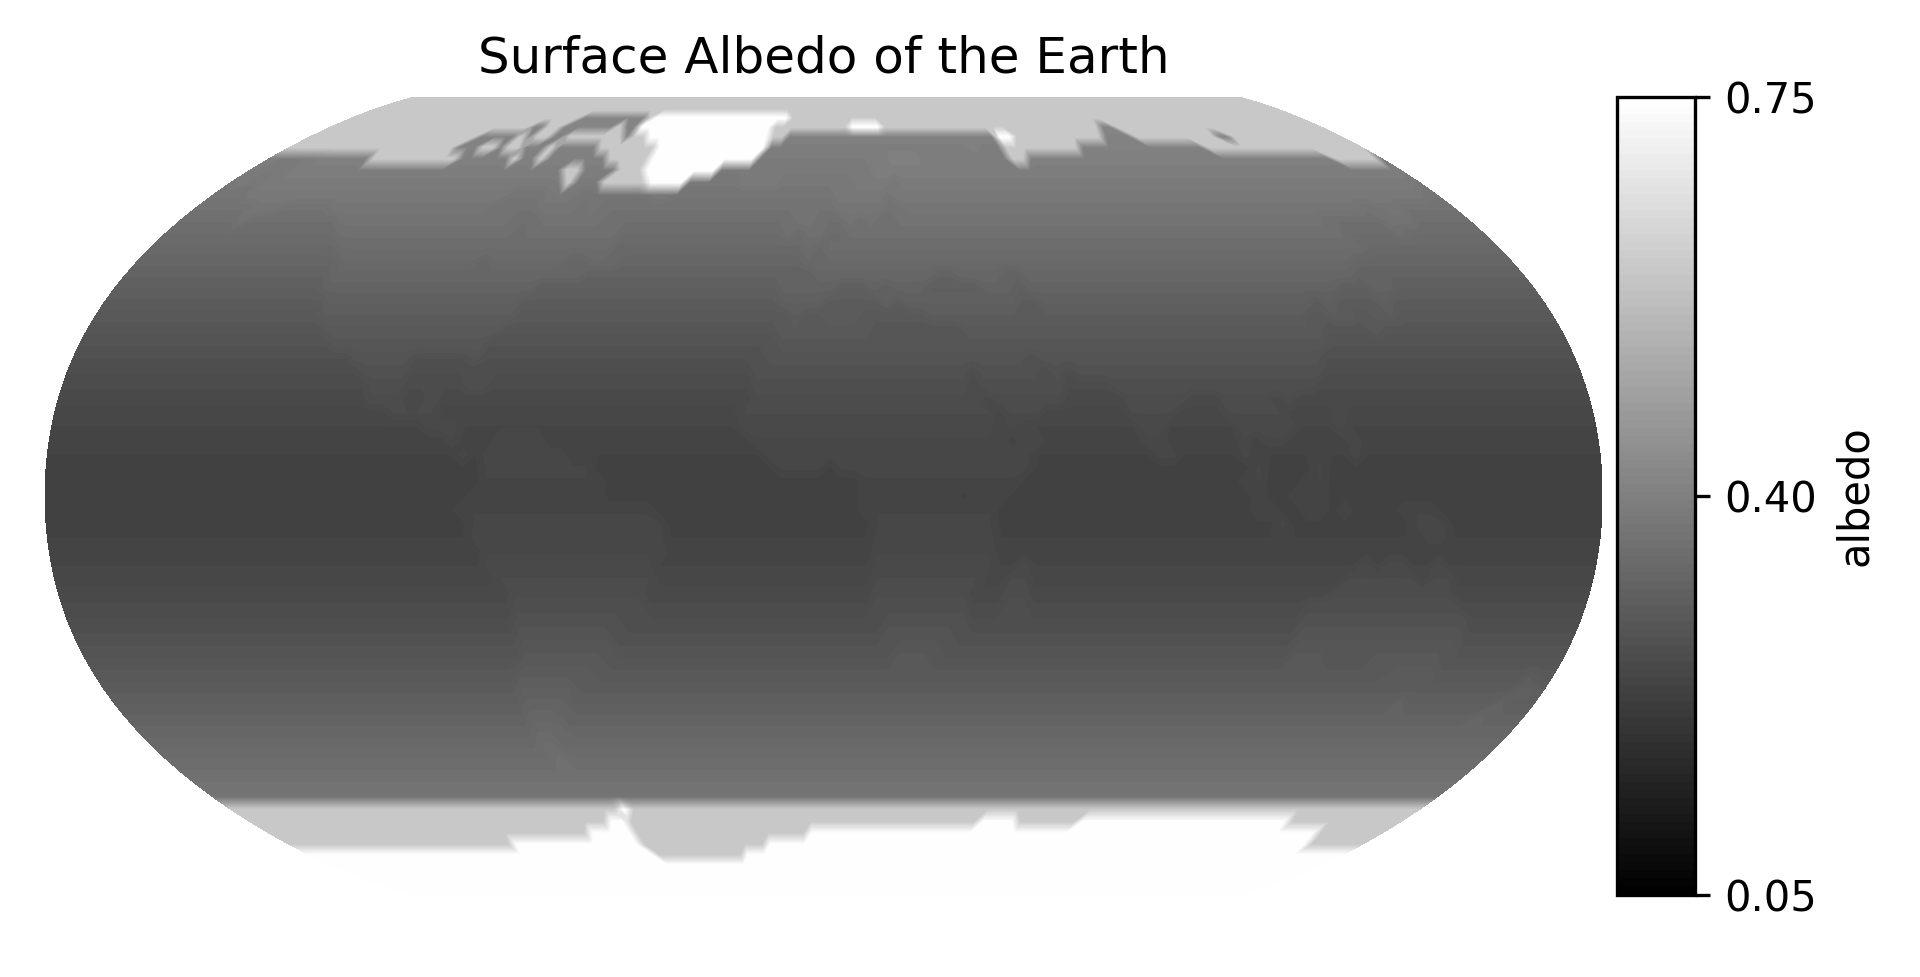
\includegraphics[width=0.72\linewidth]{figs/albedo.png}
\caption{Plot of the albedo}
\end{figure}

\begin{figure}[!htb]
	\centering
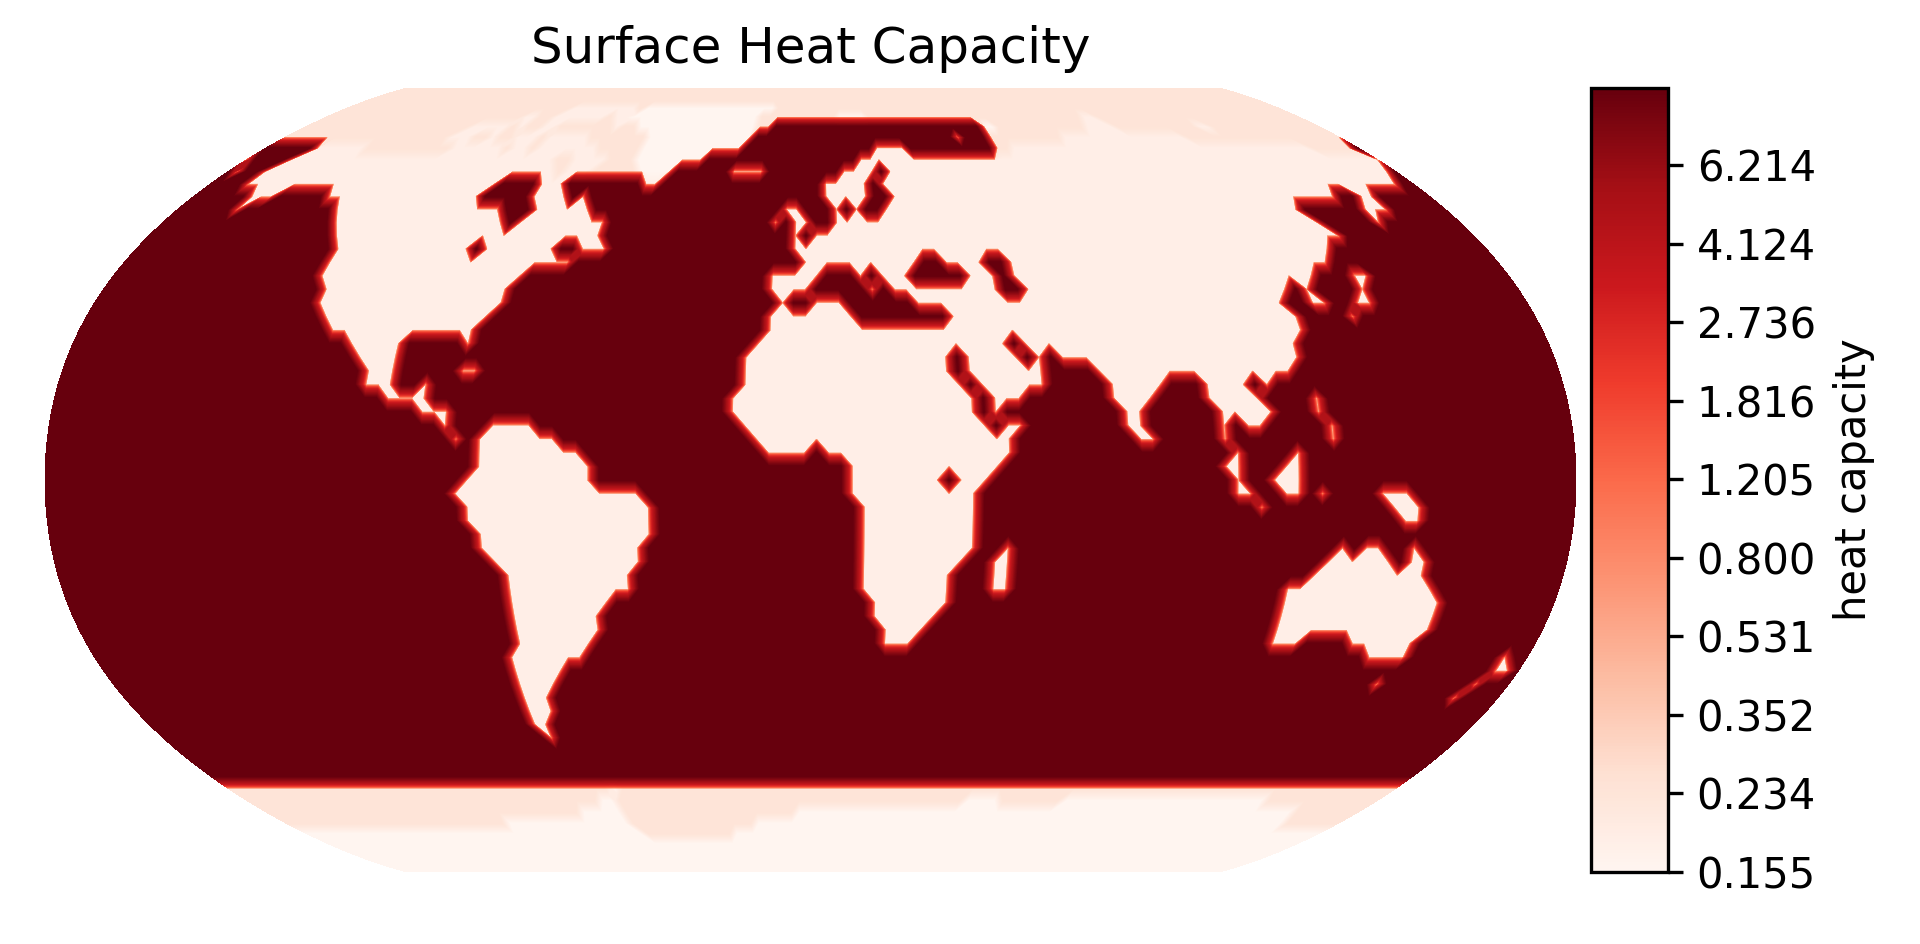
\includegraphics[width=0.72\linewidth]{figs/heat_capacity.png}
\caption{Plot of the heat capacity}
\end{figure}

\begin{figure}[!h]
\centering
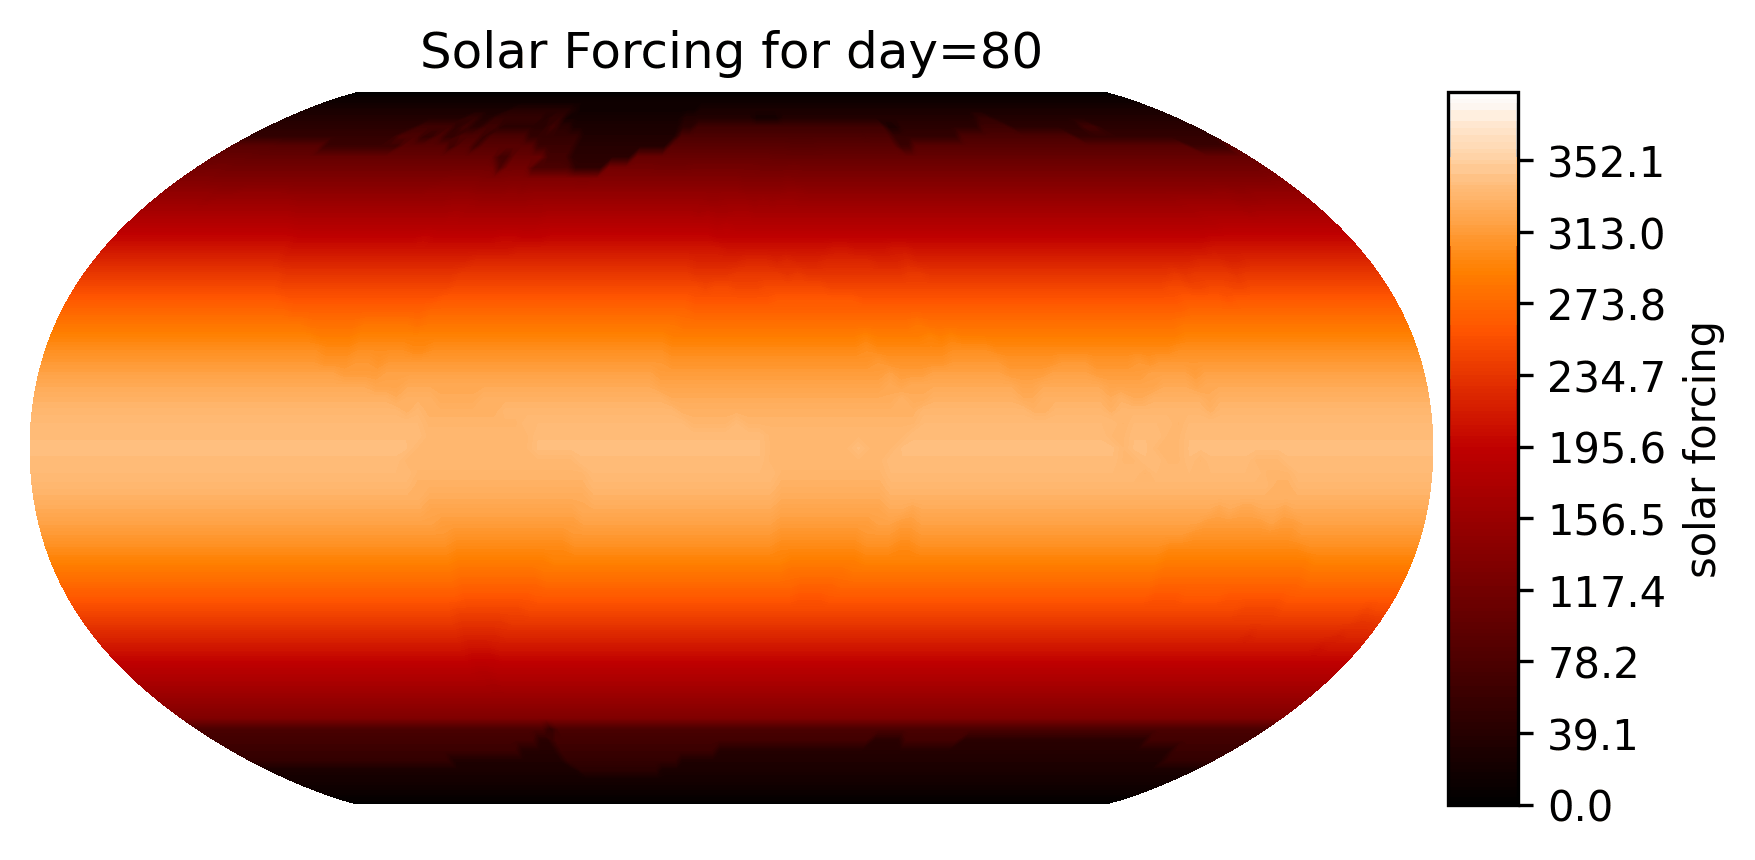
\includegraphics[width=0.72\linewidth]{figs/solar_forcing_day_80.png}
\caption{Example plot for the solar forcing on day 80 of the year}
\end{figure}
\end{document}
